%\documentclass[10pt]{beamer}
%\usetheme{amcg}
%\usepackage{subfigure}

%\begin{document}

\subsection{Advection of a top hat}

\begin{frame}
  \frametitle{Advection of a top hat}
  \begin{itemize}
  \item Top hat distribution of a tracer, advected with prescribed velocity
  \item Compares CG, CV, DG discretisations
  \item Simple, fast: run time 2 min.
  \end{itemize}

  \begin{figure}
    \centering
    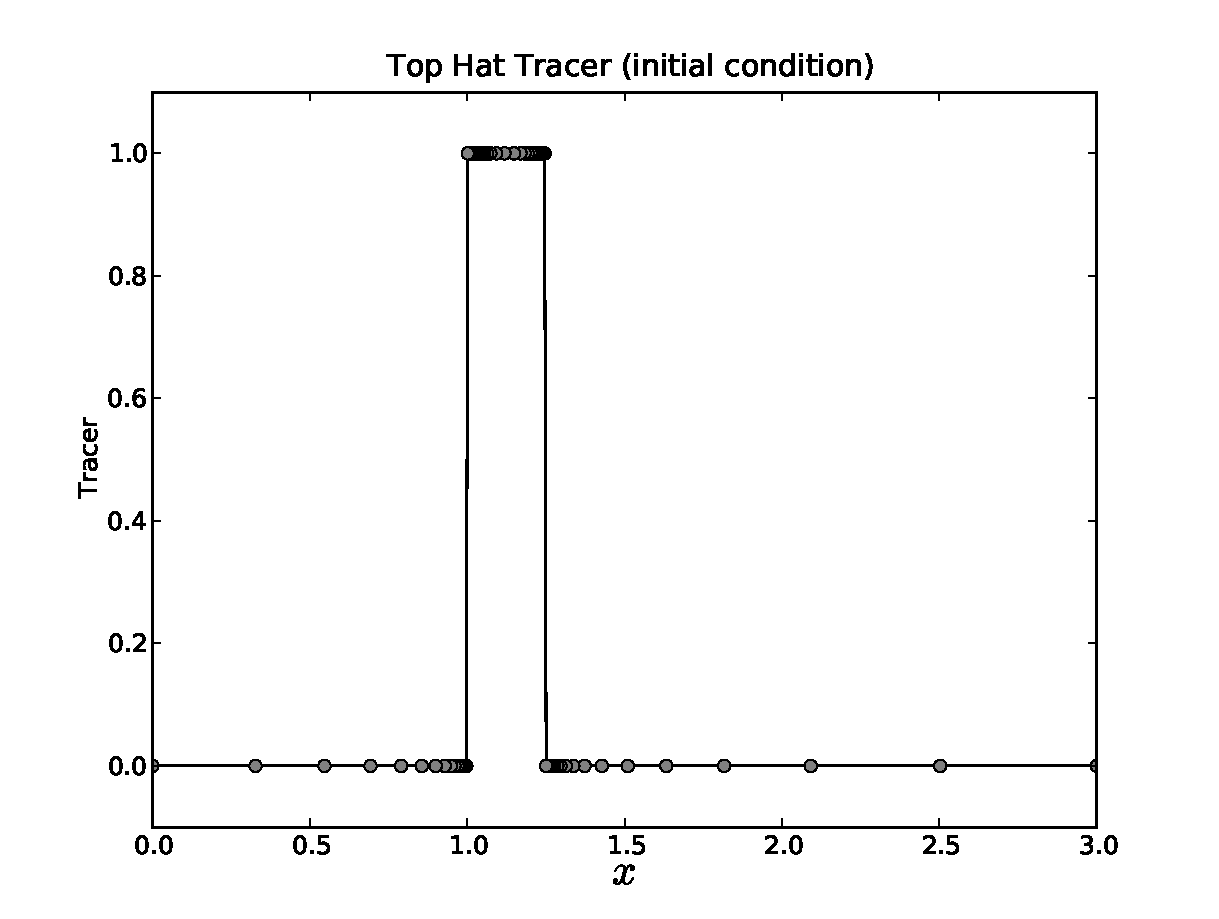
\includegraphics[width=0.45\textwidth]{./top_hat/top_hat_ic.pdf}
    \caption{Initial top hat distribution.}
  \end{figure}
\end{frame}

\begin{frame}
  \frametitle{Advection of a top hat}
  \begin{figure}[ht]
    \begin{tabular}{ccc}
      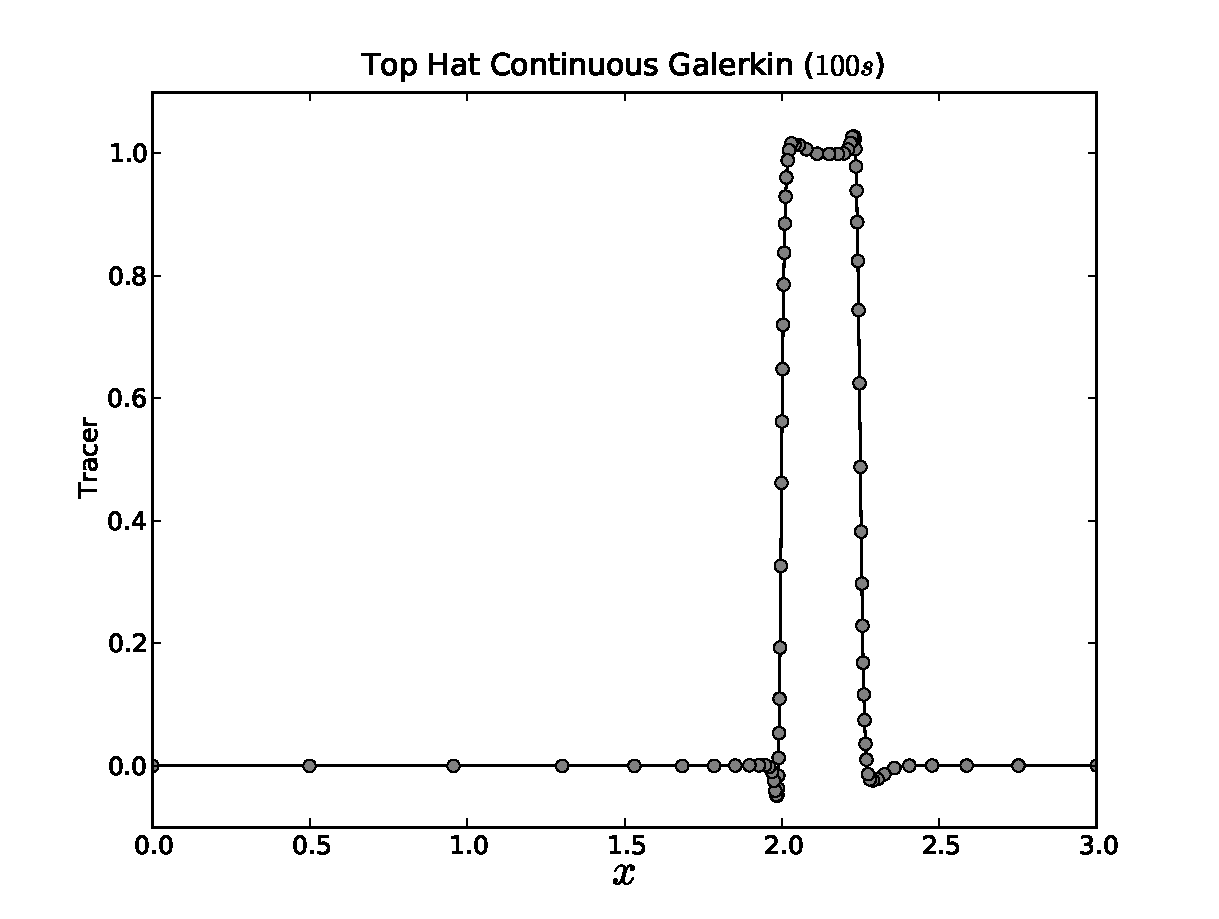
\includegraphics[width=0.3\textwidth]{./top_hat/top_hat_cg.pdf} &
      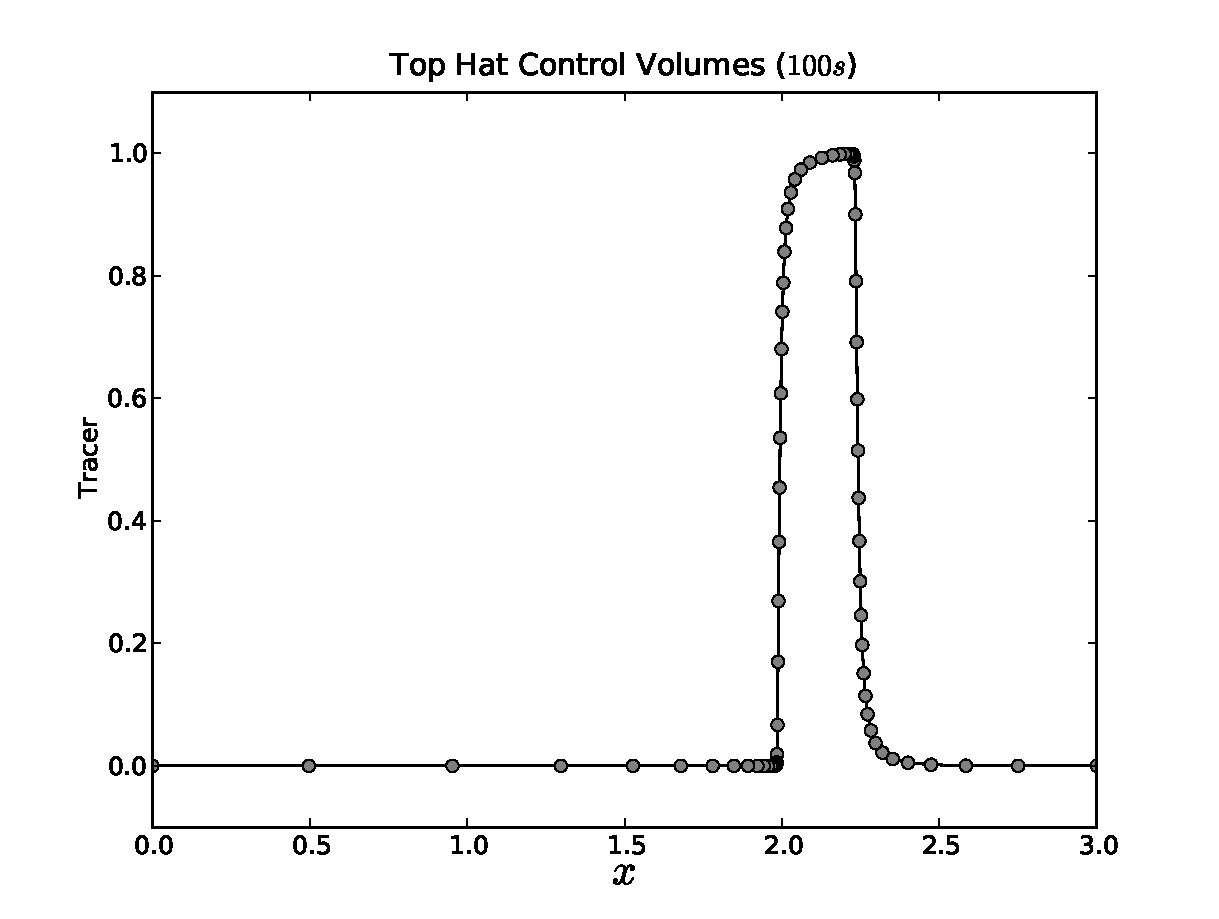
\includegraphics[width=0.3\textwidth]{./top_hat/top_hat_cv.pdf} &
      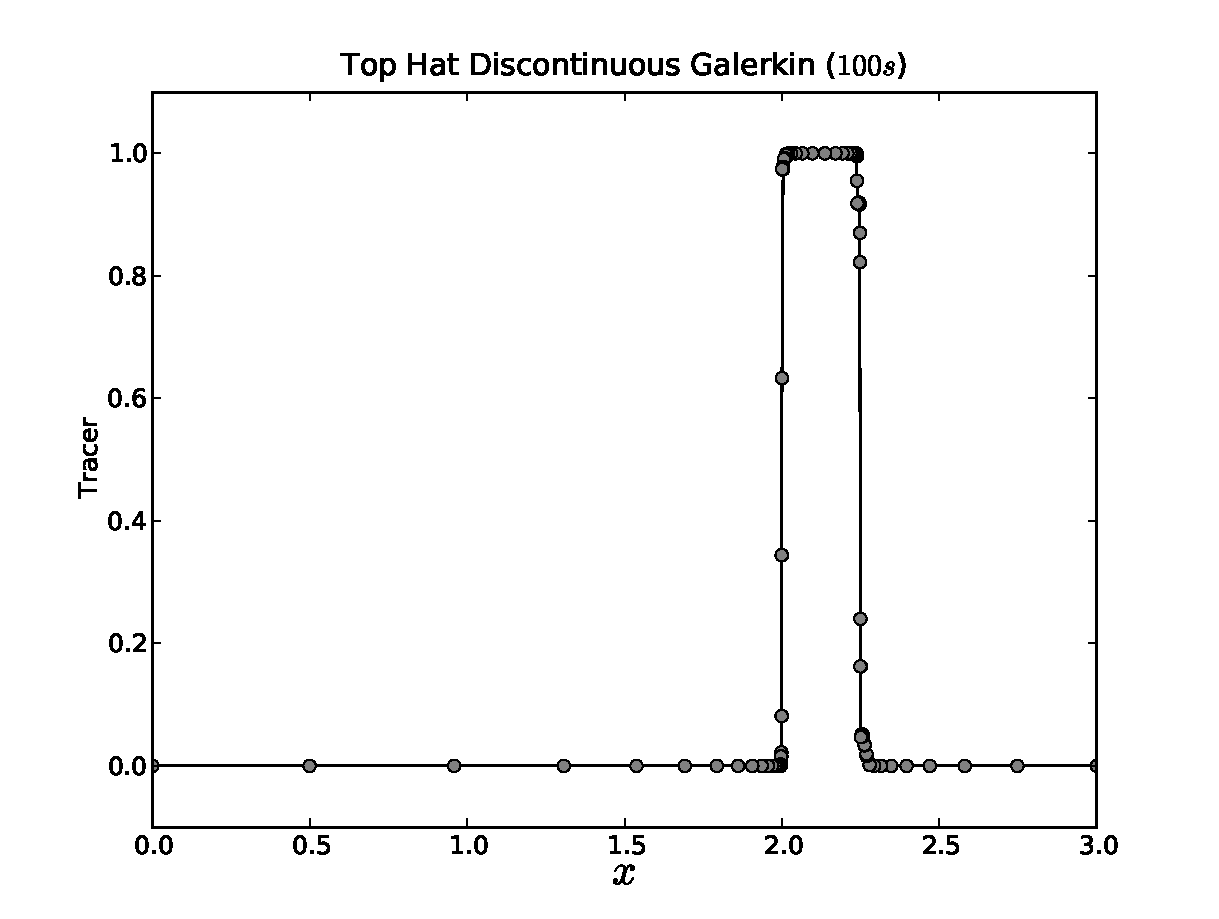
\includegraphics[width=0.3\textwidth]{./top_hat/top_hat_dg.pdf} \\
      Continuous & Control & Discontinuous  \\
       Galerkin &  Volume & Galerkin
    \end{tabular}
  \end{figure}
\end{frame}

\begin{frame}
  Continuous Galerkin
  \begin{itemize}
  \item Basic finite element discretisation
  \item Not good for advection of sharp discontinuities
  \item Not conservative
  \item SUPG stabilisation applied in this instance
  \end{itemize}
  \vspace{5pt}
  Control Volume
  \begin{itemize}
  \item Simple and efficient, sometimes diffusive
  \item Need to choose an interpolation method.  Here, `FiniteElement' interpolation with Sweby limiter is used.
  \end{itemize}
  \vspace{5pt}
  Discontinuous Galerkin
  \begin{itemize}
  \item Popular for advection problems
  \item Slope limiters still needed near discontinuities to prevent overshoots
  \end{itemize}
\end{frame}

\begin{frame}
  \frametitle{Exercises}
  \begin{itemize}
    \item Turn off SUPG stabilisation for the CG case and see what it does.
    \item Change the resolution of the adapted meshes.
    \item Change the temporal and spatial discretisations to get a less diffusive CV advection scheme.
  \end{itemize}
\end{frame}

%\end{document}
